\section{O Desafio da Causalidade e Testes Clínicos}

\begin{frame}{Associação vs. Causalidade}
    \begin{block}{O Problema da Correlação}
        Na ciência de dados, encontrar padrões associados (ex: quem toma determinado remédio se recupera mais) não garante que o remédio seja a causa da cura.
    \end{block}
    \begin{block}{Variável de Confundimento (Confounding Variable)}
        Variáveis externas não observadas que influenciam tanto a escolha do tratamento quanto o resultado de saúde (ex: renda, hábitos de exercício, gravidade inicial da dor).
    \end{block}
    \begin{columns}
        \begin{column}{0.5\textwidth}
            \begin{alertblock}{Estudo Observacional}
                Os próprios sujeitos decidem se tomam o tratamento. Alto risco de viés de confundimento.
            \end{alertblock}
        \end{column}
        \begin{column}{0.5\textwidth}
            \begin{alertblock}{Experimento Aleatório (RCT)}
                A alocação ao tratamento é decidida por sorteio aleatório, neutralizando variáveis de confundimento.
            \end{alertblock}
        \end{column}
    \end{columns}
\end{frame}

\begin{frame}{Estudo de Caso no Ceará: Dor Lombar Crônica}
    \begin{block}{O Cenário Clínico}
        Pesquisadores cearenses investigaram a eficácia do uso de \textbf{Toxina Botulínica Tipo A (BTA)} para o tratamento de dor lombar crônica persistente em pacientes atendidos no Hospital Universitário Walter Cantídio (HUWC) em Fortaleza, Ceará.
    \end{block}
    \begin{block}{Desenho do Experimento}
        \begin{itemize}
            \item Tamanho da Amostra ($N$): $31$ pacientes cearenses.
            \item \textbf{Grupo de Controle (Salina):} $16$ pacientes receberam placebo.
            \item \textbf{Grupo de Tratamento (BTA):} $15$ pacientes receberam a dose terapêutica.
            \item \textbf{Duplo-Cego:} Nem os médicos aplicadores nem os pacientes sabiam quem havia recebido BTA ou soro fisiológico.
        \end{itemize}
    \end{block}
\end{frame}

\begin{frame}{Os Resultados Experimentais}
    \begin{columns}
        \begin{column}{0.5\textwidth}
            \textbf{Resultados da Recuperação:}
            \begin{itemize}
                \item Avaliado 8 semanas após a aplicação.
                \item \textbf{Grupo de Controle:} 2 de 16 pacientes melhoraram ($12.5\%$).
                \item \textbf{Grupo de Tratamento:} 9 de 15 pacientes melhoraram ($60.0\%$).
            \end{itemize}
            \vspace{0.2cm}
            \begin{alertblock}{A Pergunta Estatística}
                A taxa de melhoria de $60\%$ contra $12.5\%$ é estatisticamente significante para provar causalidade, ou a diferença é apenas mero acaso do sorteio dos grupos?
            \end{alertblock}
        \end{column}
        \begin{column}{0.5\textwidth}
            \centering
            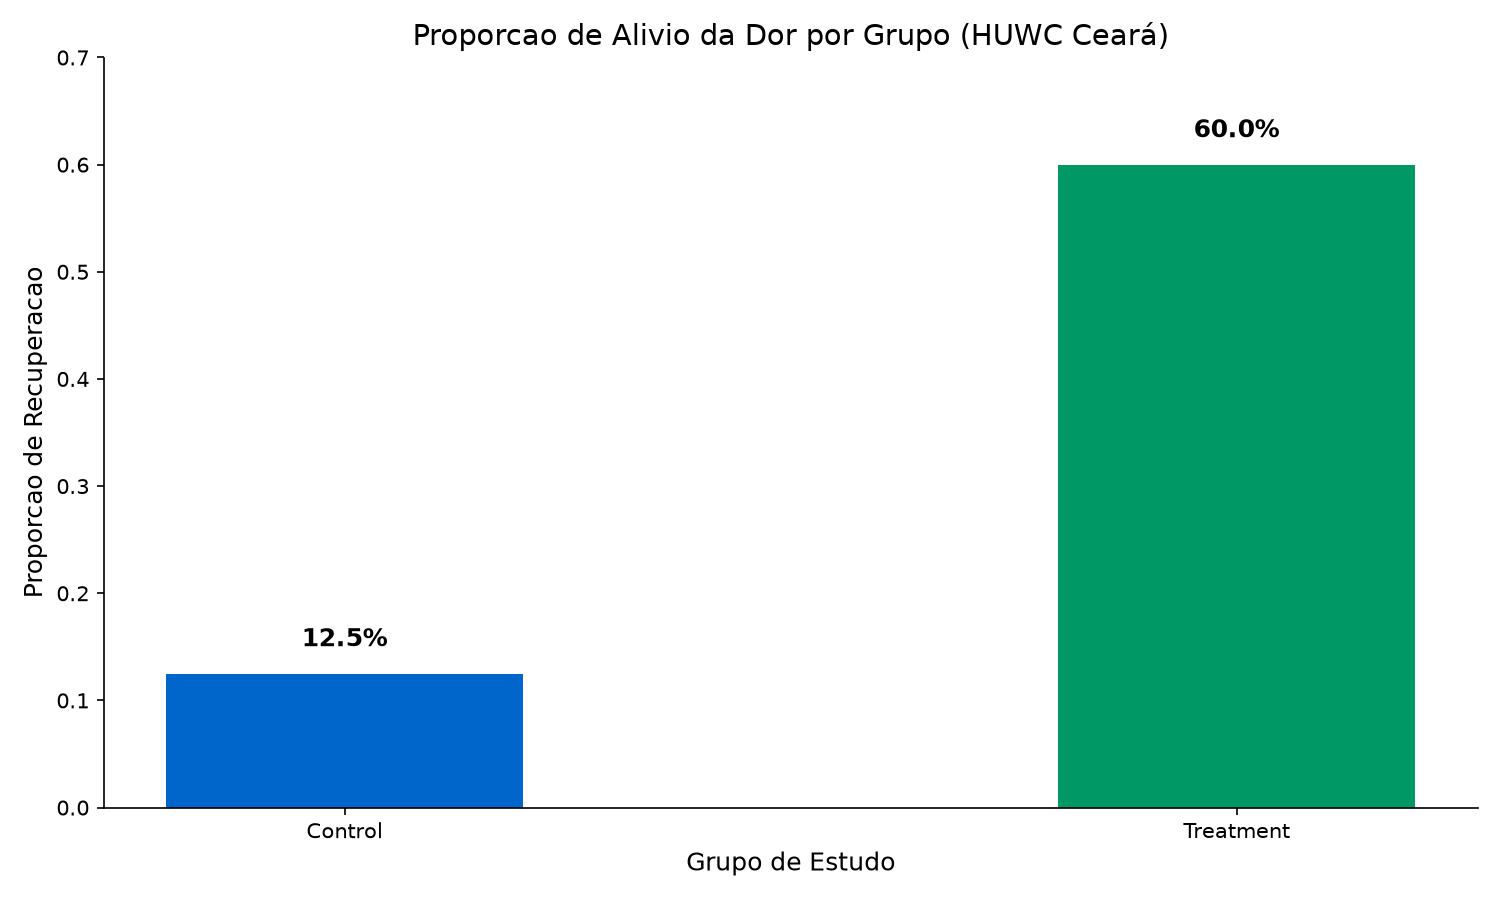
\includegraphics[width=\textwidth]{02_causalidade_barras.png}
        \end{column}
    \end{columns}
\end{frame}
